\section{Introduction}
\label{sec:intro}

Many real-world systems can be modeled by graphs, from power grids to arXiv citations to friendships on Facebook.  Early models attempted to model all systems with the same type of graph.  For example, the Erdos-Renyi random graph~\cite{erdds1959random}\cite{erdos1960random} models all networks with $n$ participants and $m$ connections with a graph of $n$ nodes and $m$ randomly placed edges.  The Watts-Strogatz model~\cite{watts1998collective} models all networks by connecting nodes to their nearest neighbors, then filling the rest of the graph with randomly placed edges.

More sophisticated models account for differences in degree distribution and clustering coefficient.  The preferential-attachment model~\cite{albert2002statistical} generates a graph with power-law degree distribution and allows the modeler to choose the exponent in the power law.  The configuration model takes as input an exact sequence of degrees and creates a random graph with that degree sequence.  Newman's "triangle-edge" model~\cite{newman2009random} generalizes this to create a random graph with specific degree sequence and clustering coefficient.

Our objective is to create a random graph with specific degree sequence and
motif counts.  (See Figure~\ref{fig:network} for an example of motif
counts.)  A motif is a small, connected subgraph of a larger graph,
and we only consider motifs with four or fewer vertices in our analysis 
(Figure~\ref{fig:motif}).  Motif counts are useful for distinguishing different
types of real-world graphs.  A network like Twitter (when converted to an
undirected graph) might have many Four
Star motifs, since a small fraction of users have large numbers of
followers who do not follow each other.  By contrast, a network like
Facebook would have a disproportionate number of Four Complete motifs, 
since a user's Facebook friends often have many mutual friends with the
user himself.  Finding the motif balance allows us to distinguish
"celebrity-based" networks from "friendship-based" networks.  (There are
also many other types of networks; email forwarding chains would have a
large number of line graphs, as would product recommendation graphs.)

\begin{figure}[t]
\centering
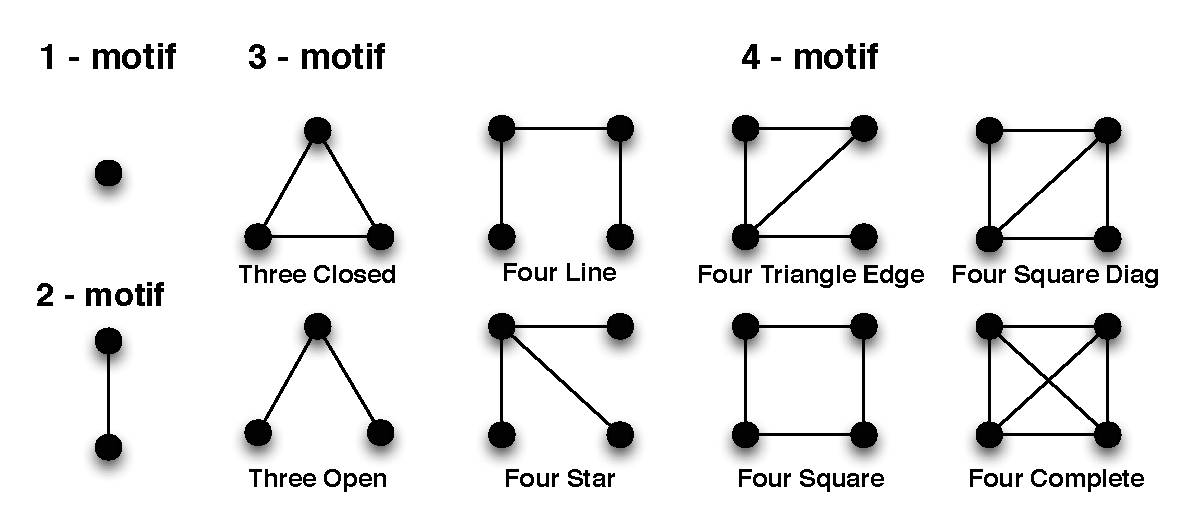
\includegraphics[width=3in]{Figures/motifs1.eps}
\caption{Graphical representation of the motifs.}
\label{fig:motif}
\end{figure}


These structures are not fully captured by models that look only at
3-motifs or clustering coefficients.  Knowing only the number of triangles
(Three Closed) and triads (Three Open), we could not tell the difference
between two strangers with one mutual friend and two strangers with two
mutual friends.  The first might correspond to two people in different
social circles who are both connected to a social "hub," while the
second might correspond to two people in the same class who know
several of the same classmates but have not yet met.  Using 4-motifs gives
us a better sense of the structure of the graph.  While
we might obtain better results by using 5- and 6-motifs, this is more
computationally intensive and we relegate it to future work.

This intuition was formalized by Chuanqi Shen, who built a classifier to
cluster networks according to their motif counts.  He found that the
clusters corresponded closely to real-life functionality~\cite{chuanqi}.
Therefore, by generating graphs with similar motif counts, we hope to build 
graphs with similar function to real-world networks.

\begin{figure}[t]
\centering
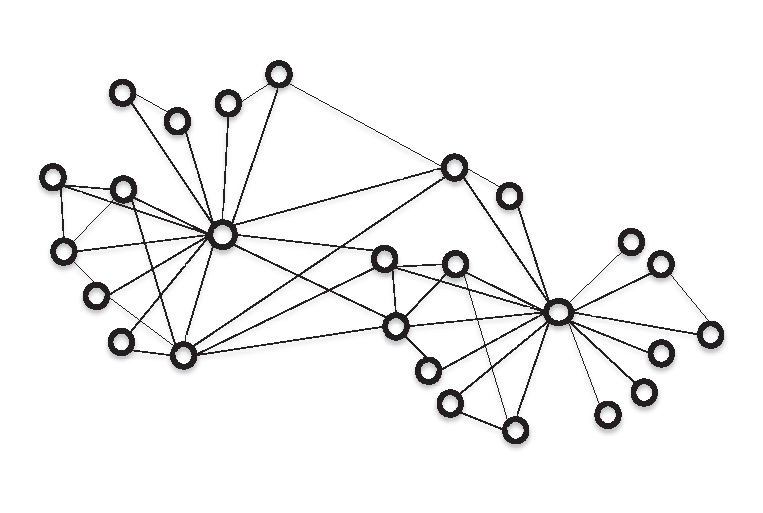
\includegraphics[width=3in]{Figures/network.eps}
\caption{A network with motif distribution \{numNodes: 25, numEdges: 44,
mtThreeClosed: 21, mtThreeOpen: 151, mfFourLine: 134,
mfFourSquare: 1, mfFourStar: 305, mfFourTriangleEdge: 155,
mfFourSquareDiag: 26, mfFourComplete: 2\}.}
\label{fig:network}
\end{figure}

%While it is difficult to find exact solutions, we use hill-climbing to find approximate solutions that produce good results in practice.

The rest of the paper is organized as follows: Section \ref{sec:problem}
formulates the problem; Section \ref{sec:related} discusses related work;
Section \ref{sec:approach-hillclimbing} describes the algorithm for
generating random graphs; Section \ref{sec:results-hillclimbing} presents 
the experimental results; Section \ref{sec:alpha} describes our method for 
predicting the degree distribution from the motif counts, and Section 
\ref{sec:futurework} describes our future work.


